% !TEX root = ../../main.tex

\chapter{Evaluation}
\label{chapter:evaluation-discussion}
This chapter shows Contribution \textbf{C.2}: A robust cost estimator for Amalur's factorized ML framework, and a comparison with the state-of-the-art in \autoref{sec:eval-model-evaluation}. Before that we show how results were collected in \autoref{sec:experiment-setup}. The \hyperref[sec:eval-discussion]{third section} of this chapter provides an in-depth interpretation of the results as well as a critical view on the implications and limitations of this work.

\section{Experiment Setup}

\label{sec:experiment-setup}

\todo{Intro experimental environment, also serves as a guide on how to replicate the results}

\subsection{Software}

\todo{Detail software packages and such}
\todo{Answer RQ.1 by showing contribution C.1 "GPU optimized implementation of Amalur’s Factorized Machine Learning frame-
    work"}


\subsection{Hardware}
\todo{Table showing different machines tested on}

\begin{table}[ht]
    \centering
    \begin{tabular}{llllp{0.19\linewidth}}
        \toprule
        Experiment & Machine        & Compute Unit & Architecture & Experiment type \\
        \midrule
        \midrule
        GPU-P-1    & WIS ST4        & GPU A40      & Ampere       & profile         \\
        GPU-P-2    & AWS P3.2xlarge & GPU V100     & Volta        & profile         \\
        GPU-P-3    & Own desktop    & GPU 1660Ti   & Turing       & profile         \\
        GPU-T-1    & DAIC           & GPU A40      & Ampere       & runtime         \\
        GPU-T-2    & DAIC           & GPU V100     & Volta        & runtime         \\
        GPU-T-3    & DAIC           & GPU P100     & Pascal       & runtime         \\
        GPU-T-4    & DAIC           & GPU 2080Ti   & Turing       & runtime         \\
        GPU-T-5    & DAIC           & GPU 1080Ti   & Pascal       & runtime         \\
        CPU-T-1    & WIS ST4        & CPU 8 cores  & -            & runtime         \\
        CPU-T-2    & WIS ST4        & CPU 16 cores & -            & runtime         \\
        CPU-T-3    & WIS ST4        & CPU 32 cores & -            & runtime         \\
        \bottomrule
    \end{tabular}
    \caption{Overview of machines experiments will be run on.}
    \label{tab:my_label}
\end{table}

\subsection{Validation Strategy}
\todo{Explain how the collected metrics are divided into separate train \& test set to test generalizability}

\begin{figure}[ht]
    \centering
    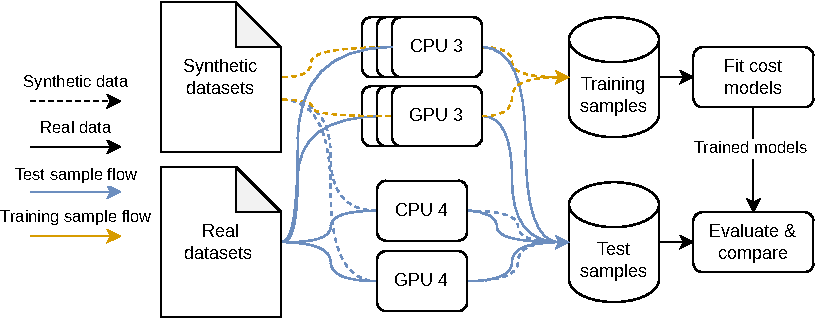
\includegraphics[width=0.8\linewidth]{chapters/06_evaluation/figures/experiment-pipeline.pdf}
    \caption{\todo{update} Overview of the planned experiments: combinations of datasets and machines we run the experiments
        on. }
    \label{fig:enter-label}
\end{figure}



\section{Cost Model Performance and Comparative Analysis}
\label{sec:eval-model-evaluation}

In this section we answer
\begin{itemize}
    \item[RQ.2] How can we accurately predict the optimal choice between factorized or materialized training of a Machine Learning model, on CPU and GPU, through leveraging knowledge about model, data, and hardware characteristics?
\end{itemize}

\subsection{Exploring Generalizability}
\subsubsection{Performance with New Datasets}

\subsubsection{Ablation Study}


\subsection{Cost Estimator Comparison}


\section{Discussion}
\label{sec:eval-discussion}

